%%%%%%%%%%%%%%%%%%%%%%%%%%%%%%%%%%%%%%%%%
% Beamer Presentation
% LaTeX Template
% Version 1.0 (10/11/12)
%
% This template has been downloaded from:
% http://www.LaTeXTemplates.com
%
% License:
% CC BY-NC-SA 3.0 (http://creativecommons.org/licenses/by-nc-sa/3.0/)
%
%%%%%%%%%%%%%%%%%%%%%%%%%%%%%%%%%%%%%%%%%

%----------------------------------------------------------------------------------------
%	PACKAGES AND THEMES
%----------------------------------------------------------------------------------------

\documentclass{beamer}

\mode<presentation> {

% The Beamer class comes with a number of default slide themes
% which change the colors and layouts of slides. Below this is a list
% of all the themes, uncomment each in turn to see what they look like.

%\usetheme{default}
%\usetheme{AnnArbor}
%\usetheme{Antibes}
%\usetheme{Bergen}
\usetheme{Berkeley}
%\usetheme{Berlin}
%\usetheme{Boadilla}
%\usetheme{CambridgeUS}
%\usetheme{Copenhagen}
%\usetheme{Darmstadt}
%\usetheme{Dresden}
%\usetheme{Frankfurt}
%\usetheme{Goettingen}
%\usetheme{Hannover}
%\usetheme{Ilmenau}
%\usetheme{JuanLesPins}
%\usetheme{Luebeck}
%\usetheme{Madrid}
%\usetheme{Malmoe}
%\usetheme{Marburg}
%\usetheme{Montpellier}
%\usetheme{PaloAlto}
%\usetheme{Pittsburgh}
%\usetheme{Rochester}
%\usetheme{Singapore}
%\usetheme{Szeged}
%\usetheme{Warsaw}

% As well as themes, the Beamer class has a number of color themes
% for any slide theme. Uncomment each of these in turn to see how it
% changes the colors of your current slide theme.

%\usecolortheme{albatross}
%\usecolortheme{beaver}
%\usecolortheme{beetle}
%\usecolortheme{crane}
%\usecolortheme{dolphin}
\usecolortheme{dove} %fine
%\usecolortheme{fly}
%\usecolortheme{lily}
%\usecolortheme{orchid}
%\usecolortheme{rose}
%\usecolortheme{seagull}
%\usecolortheme{seahorse}
%\usecolortheme{whale}
%\usecolortheme{wolverine}

%\setbeamertemplate{footline} % To remove the footer line in all slides uncomment this line
\setbeamertemplate{footline}[page number] % To replace the footer line in all slides with a simple slide count uncomment this line

\setbeamertemplate{navigation symbols}{} % To remove the navigation symbols from the bottom of all slides uncomment this line
}

\usepackage{graphicx} % Allows including images
\usepackage{booktabs} % Allows the use of \toprule, \midrule and \bottomrule in tables

\usepackage{subcaption}
%\usepackage{enumitem}

%\setlist[itemize,2]{label={$\star$}}

%----------------------------------------------------------------------------------------
%	TITLE PAGE
%----------------------------------------------------------------------------------------

\title[TCP Measurements]{TCP Measurements} % The short title appears at the bottom of every slide, the full title is only on the title page

\author{Jiri Hamberg} % Your name
\institute[Uni.Helsinki] % Your institution as it will appear on the bottom of every slide, may be shorthand to save space
{
University of Helsinki \\ % Your institution for the title page
\medskip
\textit{jiri.hamberg@cs.helsinki.fi} % Your email address
}
\date{15.12.2016} % Date, can be changed to a custom date

\begin{document}

\begin{frame}
\titlepage % Print the title page as the first slide
\end{frame}

\begin{frame}
\frametitle{Overview} % Table of contents slide, comment this block out to remove it
\tableofcontents % Throughout your presentation, if you choose to use \section{} and \subsection{} commands, these will automatically be printed on this slide as an overview of your presentation
\end{frame}

%----------------------------------------------------------------------------------------
%	PRESENTATION SLIDES
%----------------------------------------------------------------------------------------

%------------------------------------------------
\section{Introduction} 

\begin{frame}
\frametitle{Introduction}

\begin{itemize}
	\item Why should we measure TCP?
	\setbeamertemplate{itemize items}[circle]	
	\begin{itemize}
		\item TCP is the backbone of the Internet
		
		\item TCP needs to keep up with evolving Internet
	\end{itemize}
\end{itemize}

\end{frame}


\section{Metrics}

\begin{frame}
\frametitle{Metrics}
\begin{itemize}
	\item Throughput (and goodput)
	\item Fairness
	\item Latency
	\item Loss Rate
	\item Burstiness	
\end{itemize}
\end{frame}

\begin{frame}
\frametitle{Throughput and Goodput}
\textbf{Throughput}: the amount of data transferred in a unit of time\\~\\

\textbf{Goodput}: the amount of payload transferred in a unit of time
\end{frame}

\begin{frame}
\frametitle{Fairness}
Intuitively, fairness means that resources are distributed evenly\\~\\

Jain et al. (1984)
\begin{equation*}
f(\textbf{x}) = \frac{ \left(\sum\limits_{i=1}^{n} x_i\right)^2 }{n \sum\limits_{i=1}^{n} x_i^2 } 
\end{equation*}

\begin{itemize}
	\item Scale independent
	\item Bounded
	\item Continuous
\end{itemize}

\end{frame}

\begin{frame}
\frametitle{Other Metrics}

Latency\\~\\

Loss Rate\\~\\

Burstiness\\~\\

\end{frame}

\section{Measurement Platforms}

\begin{frame}
\frametitle{Measurement Platforms}

Measurement platforms offer different ways to set up experiments

\begin{itemize}
	\item Testbed
	\item Live Internet Test
	\item Simulation
	\item Emulation
\end{itemize}
\end{frame}

\begin{frame}
\frametitle{Testbed}
Testbed is an isolated network where experiments can be conducted
\begin{itemize}
	\item Provides total control over the experiment - no interference
	\item Does not scale well
\end{itemize}

\end{frame}

\begin{frame}
\frametitle{Live Internet Test}
Use a mesh geographically distributed hosts for conducting measurements
\begin{itemize}
	\item Can measure on $O(n^2)$ network paths with $n$ hosts
	\item Inexpensive and realistic results
	\item Hard to control and measure the network paths 
\end{itemize}

\end{frame}

\begin{frame}
\frametitle{Simulation}
Use a scriptable general purpose simulation framework or write your own

\begin{itemize}
	\item Cheap, fast and scalable
	\item Lose some details compared to conventional measurements
	\item Results may require validation with real experiments
\end{itemize}

\end{frame}

\begin{frame}
\frametitle{Emulation}
Combination of simulation with other techniques
\begin{itemize}
	\item Simulate part of the network that cannot easily included in the experiment or does not exist yet
\end{itemize}

\end{frame}

\section{Evaluating Congestion Control Algorithms}

\begin{frame}
\frametitle{Evaluating Popular Congestion Control Algorithms}
The study used ns2 network simulations to evaluate goodput and fairness common TCP congestion control algorithms\\~\\

Algorithms evaluated
\begin{itemize}
	\item New Reno
	\item Compound
	\item Cubic
\end{itemize}

Wired and wireless connections were simulated
\end{frame}

\begin{frame}
\frametitle{New Reno}
Default congestion control implementation of some versions of OSX\\~\\

TCP Reno implements the fast recovery algorithm
\begin{itemize}
	\item 3 duplicate ACKs trigger a re-transmission\\~\\
\end{itemize}

New Reno improves the fast recovery algorithm by being able to handle multiple packet drops in a single congestion window with only one window reduction
\end{frame}

\begin{frame}
\frametitle{Compound}
Introduced in Windows Vista and Windows Server 2008\\~\\

Maintains exponentially smoothed estimate of the RTT 
\begin{itemize}
	\item Estimate is used in calculating the current window size during TCP startup
	\item Congestion window consists of two components: the regular congestion window and a RTT based component
	\item Conjoined effect is approximately
	\[
		win(t + 1) = win(t) + \alpha * win(t)^k
	\]
	when no packet loss or early congestion is detected, and
	\[
		win(t + 1) = win(t) * (1 - \beta)
	\]	
	otherwise
	  
\end{itemize}

\end{frame}

\begin{frame}
\frametitle{Cubic}
The default congestion control implementation of Linux kernel  from version 2.6.19 onwards\\~\\

Cubic replaces slow start and congestion avoidance phase with a single phase where the congestion window is given by the following formula

\[
W_{cubic}(t) = C(t - K)^3 + W_{max}   
\]

where $K = (W_{max} \beta / C)^{1 / 3}$, $W_{max}$ is the largest window size before last window reduction and $C$ and $\beta$ are free parameters.

\end{frame}

\begin{frame}
\frametitle{Wired Simulation: Goodput}


\begin{figure}
	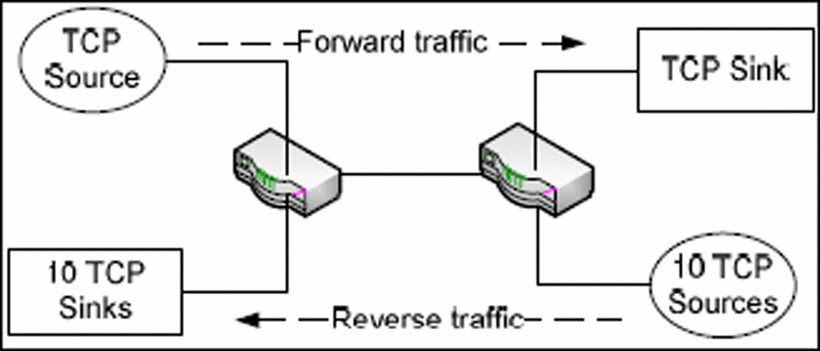
\includegraphics[width=0.5\textwidth]{images/abdeljaouad10_topology_1.png}
	\caption{Topology of the wired ns2 simulation}
\end{figure}

\begin{table}
\small
\begin{tabular}{l*{3}{c}l}
& Compound & Cubic & New Reno & Rev. Traffic \\
\hline
0s-250s Mbps & 1.99 & 1.99 & 1.98 & No \\
250s-500s Mbps & 1.79 & 1.96 & 1.71 & Yes \\
500s-750s Mbps & 2.00 & 2.00 & 1.99 & No \\
750s-1000s Mbps & 1.80 & 1.96 & 1.76 & Yes \\
\end{tabular}
\caption{Goodput achieved by each TCP variant with and without reverse traffic at different time intervals.}
\end{table}

\end{frame}

\begin{frame}
\frametitle{Wired Simulation: Fairness}
\begin{figure}
	%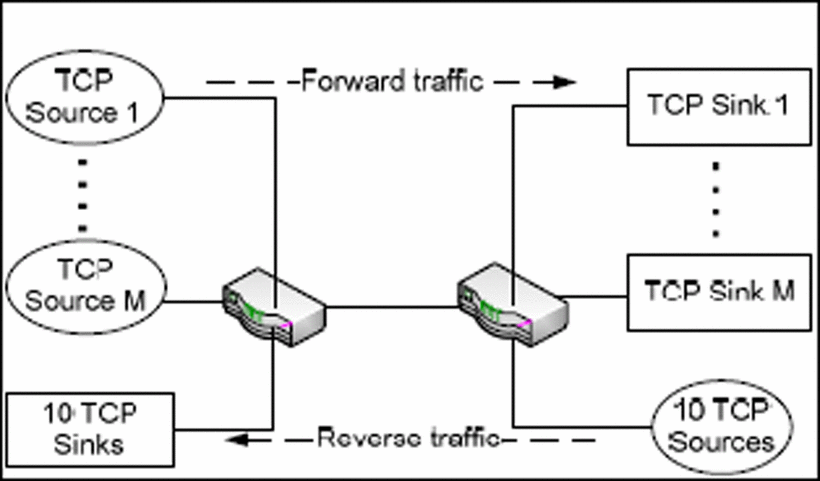
\includegraphics[width=0.5\textwidth]{images/abdeljaouad10_topology_2.png}
	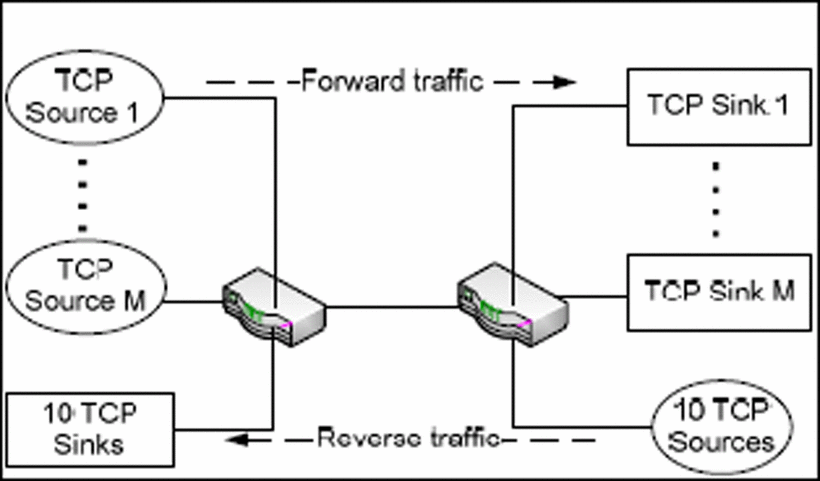
\includegraphics[height=0.3\textheight]{images/abdeljaouad10_topology_2.png}
	\caption{Network topology in measuring fairness}
	%\label{fig:topology2}
\end{figure}

\begin{figure}
	%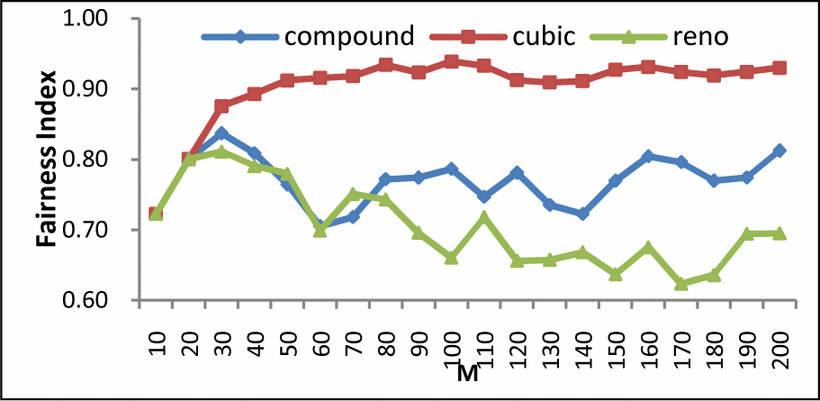
\includegraphics[width=0.5\textwidth]{images/abdeljaouad10_fairness_1.png}
	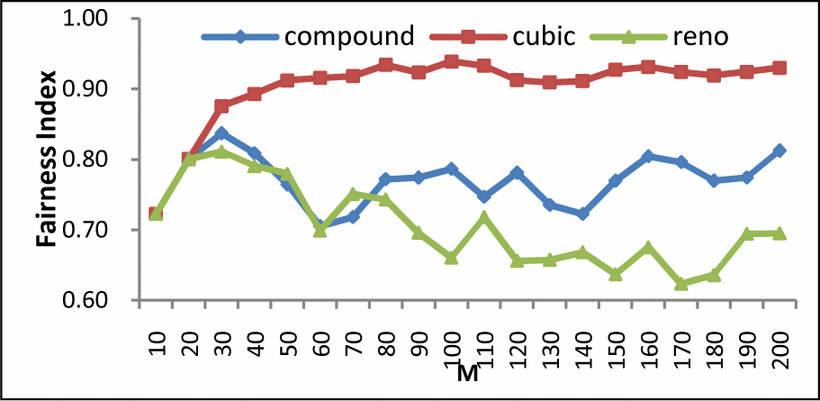
\includegraphics[height=0.3\textheight]{images/abdeljaouad10_fairness_1.png}
	\caption{Fairness of TCP variants as a function of concurrent senders}
	%\label{fig:fairness1}
\end{figure}
\end{frame}

\begin{frame}
\frametitle{Wireless Simulation}
\begin{figure}
	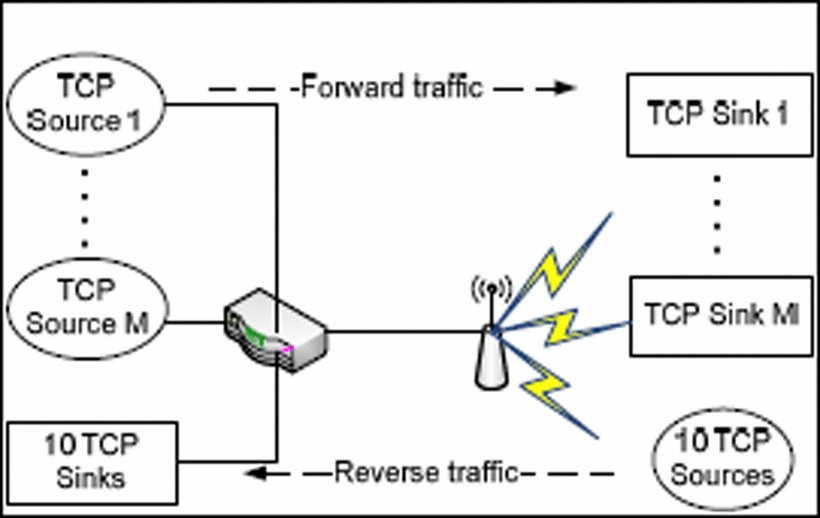
\includegraphics[height=0.3\textheight]{images/abdeljaouad10_topology_3.png}
	\caption{Topology of the wireless ns2 simulation}
	%\label{fig:topology3}
\end{figure}


%\begin{figure}
%	 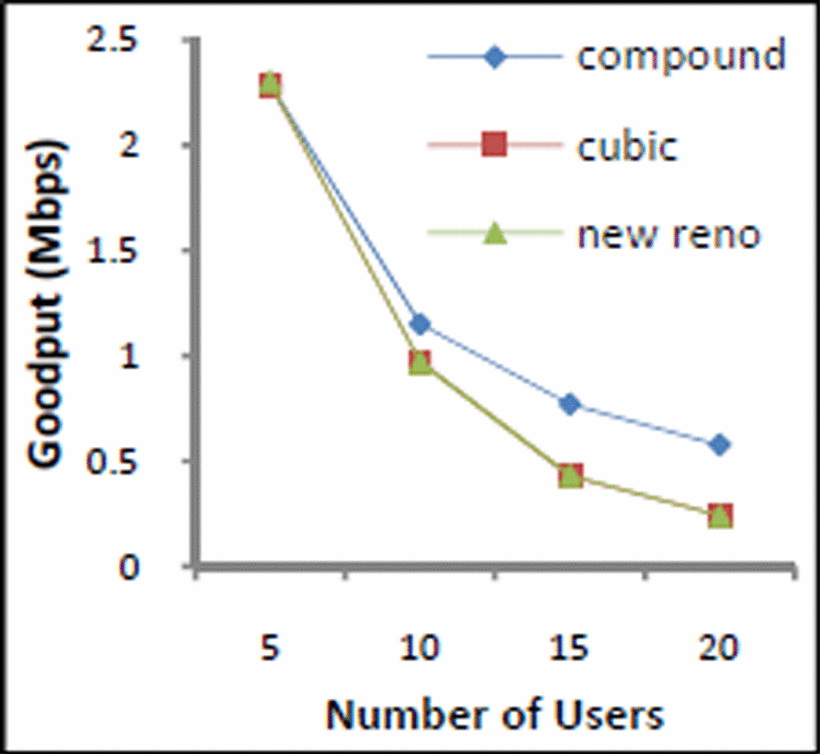
\includegraphics[height=0.3\textheight]{images/abdeljaouad10_goodput.png}
%	\caption{Goodput as a function of the number of concurrent connections} %\label{fig:goodput}
%\end{figure}

\begin{figure}
\centering
\begin{subfigure}{.5\textwidth}
 	\centering
  	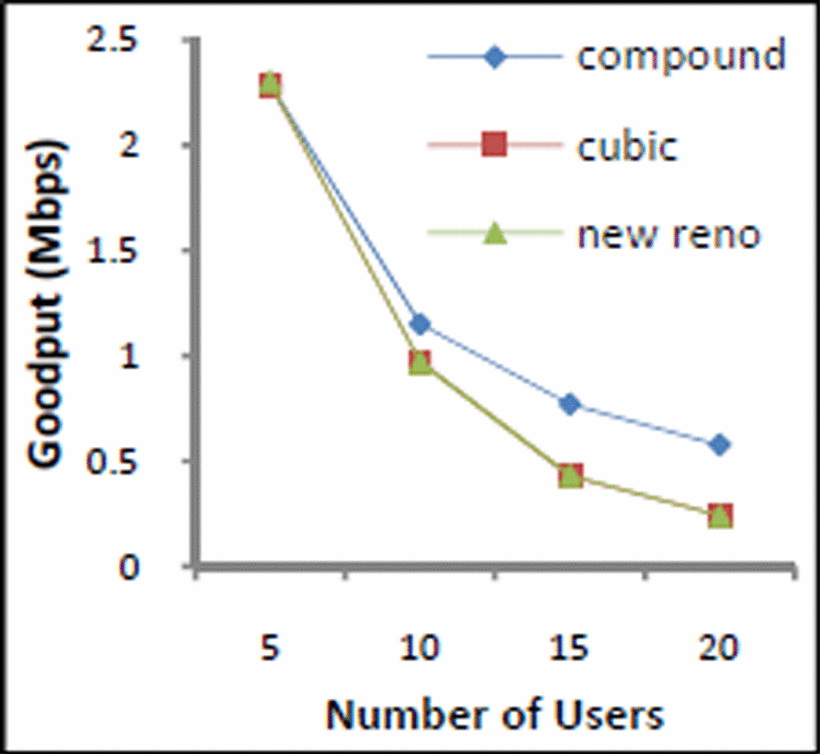
\includegraphics[width=.65\linewidth]{images/abdeljaouad10_goodput.png}
  	\caption{Goodput}
  	%\label{fig:sub1}
\end{subfigure}%
\begin{subfigure}{.5\textwidth}
 	\centering
  	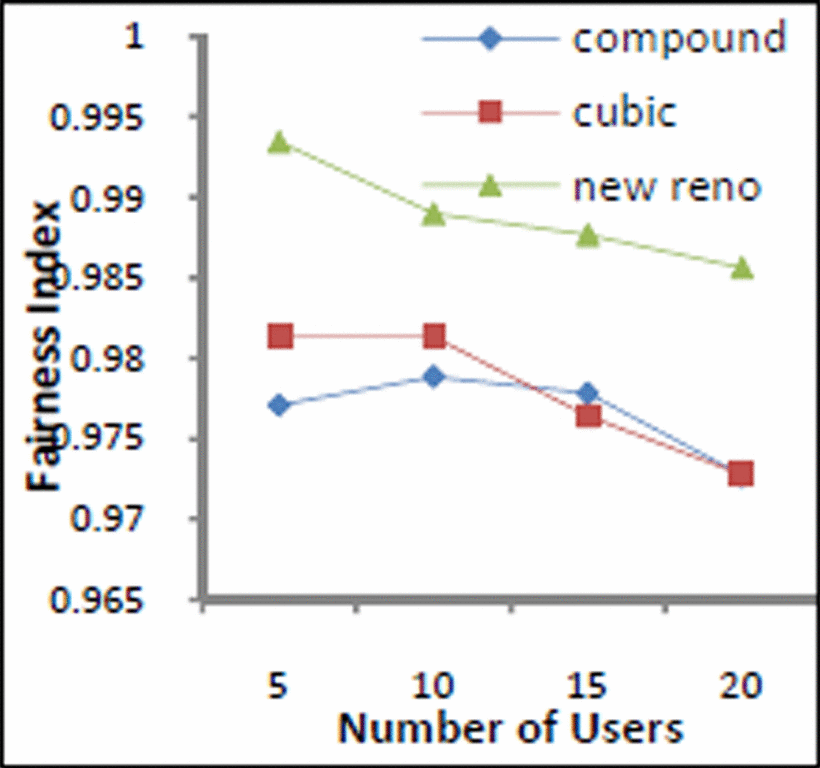
\includegraphics[width=.65\linewidth]{images/abdeljaouad10_fairness_2.png}
  	\caption{Fairness}
  	%\label{fig:sub2}
\end{subfigure}
%\caption{A figure with two subtitles}
\end{figure}

\end{frame}


\section{Improving TCP Startup Performance Using Active Measurements}

\begin{frame}
\frametitle{Improving TCP Startup Performance Using Active Measurements}
Study introduces a novel TCP startup algorithm, \textit{paced start}
\begin{itemize}
	\item Estimates the available bandwidth using \textit{Packet Transmission Rate} (PTR) method\\~\\
\end{itemize}

\textit{Paced start} is compared with the \textit{slow start}
\begin{itemize}
	\item Simulations with ns2
	\item Measurements on the Emulab testbed
\end{itemize}

\end{frame}

\begin{frame}
\frametitle{Paced Start}
\begin{figure}
	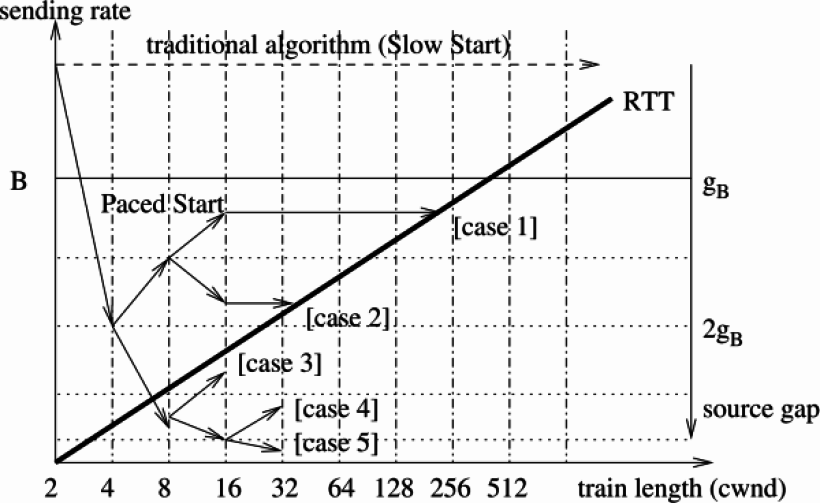
\includegraphics[width=0.8\textwidth]{images/hu03_paced_start_search.png}
	\caption{Slow start algorithm moves along the X-axis until a suitably large cwnd is found (or ssthresh is hit). Paced start also considers the Y-axis, doing a binary search to find the suitable sending rate}
	%\label{fig:paced_start}
\end{figure}
\end{frame}

\begin{frame}
\frametitle{Paced Start and Slow Start}
\begin{figure}
	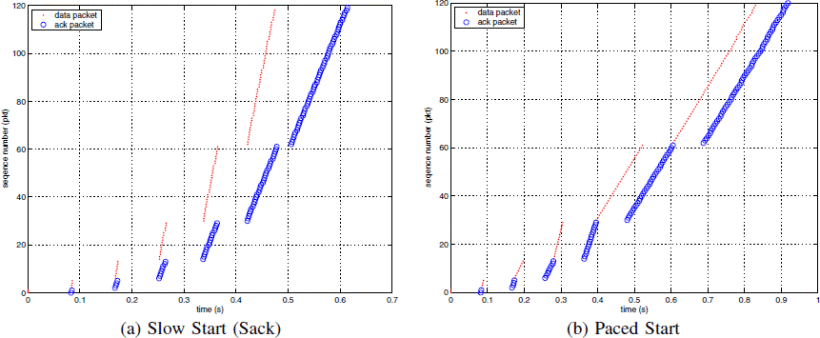
\includegraphics[width=0.8\textwidth]{images/hu03_PTR.png}
	\caption{Packet trains of source and target machines plotted against time for both slow start and paced start algorithm (simulation)}
	%\label{fig:PTR}
\end{figure}
\end{frame}

\begin{frame}
\frametitle{Evaluation Using Simulation}
	\begin{figure}
	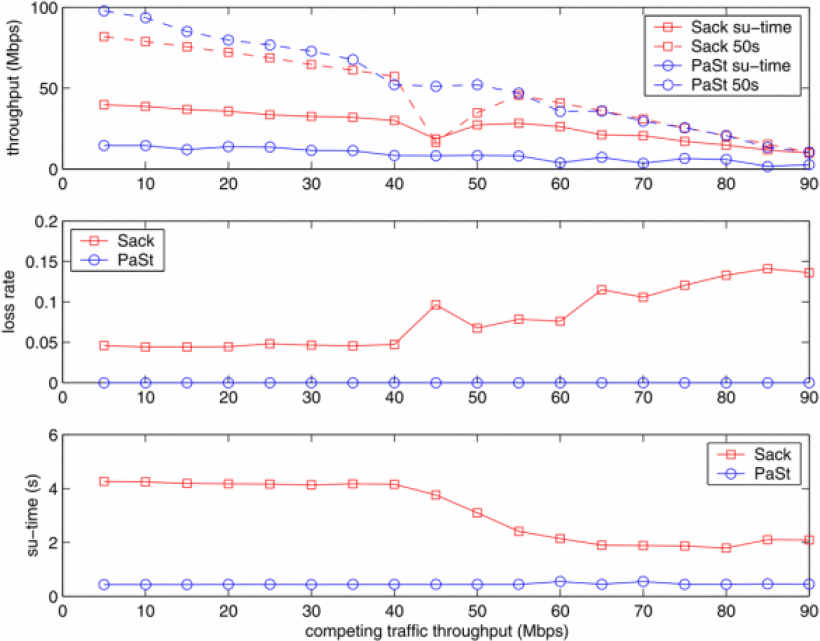
\includegraphics[width=0.5\textwidth]{images/hu03_competing_traffic.png}
	\caption{The effect of competing traffic on the performance of slow start (Sack) and paced start (PaSt) algorithms. ns2 network simulation.}
	%\label{fig:competing_traffic}
\end{figure}
\end{frame}

\begin{frame}
\frametitle{Evaluation UsingTestbed}
\begin{figure}
	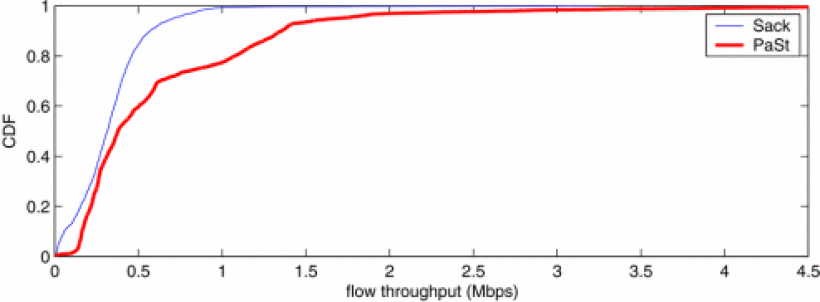
\includegraphics[width=0.5\textwidth]{images/hu03_in_kernel.png}
	\caption{Cumulative distribution functions of flow throughput during a 500 second experiment conducted on a Emulab testbed}
	%\label{fig:in_kernel}
\end{figure}

\end{frame}

\section{Conclusion}


\begin{frame}
\frametitle{Conclusion}
\begin{itemize}
	\item Measurements are useful for evaluating and improving the TCP protocol
	\item Useful metrics include goodput, fairness and latency
	\item Various ways to set up an experiment, each with pros and cons
\end{itemize}
\end{frame}


\begin{frame}
\frametitle{The End}
Thank you!
	
Questions?
\end{frame}

%\begin{frame}
%\frametitle{Paragraphs of Text}
%Sed iaculis dapibus gravida. Morbi sed tortor erat, nec interdum arcu. Sed id lorem lectus. Quisque viverra augue id sem ornare non aliquam nibh tristique. Aenean in ligula nisl. Nulla sed tellus ipsum. Donec vestibulum ligula non lorem vulputate fermentum accumsan neque mollis.\\~\\

%Sed diam enim, sagittis nec condimentum sit amet, ullamcorper sit amet libero. Aliquam vel dui orci, a porta odio. Nullam id suscipit ipsum. Aenean lobortis commodo sem, ut commodo leo gravida vitae. Pellentesque vehicula ante iaculis arcu pretium rutrum eget sit amet purus. Integer ornare nulla quis neque ultrices lobortis. Vestibulum ultrices tincidunt libero, quis commodo erat ullamcorper id.
%\end{frame}

%------------------------------------------------

%\begin{frame}
%\frametitle{Bullet Points}
%\begin{itemize}
%\item Lorem ipsum dolor sit amet, consectetur adipiscing elit
%\item Aliquam blandit faucibus nisi, sit amet dapibus enim tempus eu
%\item Nulla commodo, erat quis gravida posuere, elit lacus lobortis est, quis porttitor odio mauris at libero
%\item Nam cursus est eget velit posuere pellentesque
%\item Vestibulum faucibus velit a augue condimentum quis convallis nulla gravida
%\end{itemize}
%\end{frame}

%------------------------------------------------

%\begin{frame}
%\frametitle{Blocks of Highlighted Text}
%\begin{block}{Block 1}
%Lorem ipsum dolor sit amet, consectetur adipiscing elit. Integer lectus nisl, ultricies in feugiat rutrum, porttitor sit amet augue. Aliquam ut tortor mauris. Sed volutpat ante purus, quis accumsan dolor.
%\end{block}

%\begin{block}{Block 2}
%Pellentesque sed tellus purus. Class aptent taciti sociosqu ad litora torquent per conubia nostra, per inceptos himenaeos. Vestibulum quis magna at risus dictum tempor eu vitae velit.
%\end{block}

%\begin{block}{Block 3}
%Suspendisse tincidunt sagittis gravida. Curabitur condimentum, enim sed venenatis rutrum, ipsum neque consectetur orci, sed blandit justo nisi ac lacus.
%\end{block}
%\end{frame}

%------------------------------------------------

%\begin{frame}
%\frametitle{Multiple Columns}
%\begin{columns}[c] % The "c" option specifies centered vertical alignment while the "t" option is used for top vertical alignment

%\column{.45\textwidth} % Left column and width
%\textbf{Heading}
%\begin{enumerate}
%\item Statement
%\item Explanation
%\item Example
%\end{enumerate}

%\column{.5\textwidth} % Right column and width
%Lorem ipsum dolor sit amet, consectetur adipiscing elit. Integer lectus nisl, ultricies in feugiat rutrum, porttitor sit amet augue. Aliquam ut tortor mauris. Sed volutpat ante purus, quis accumsan dolor.

%\end{columns}
%\end{frame}

%\begin{frame}
%\frametitle{Table}
%\begin{table}
%\begin{tabular}{l l l}
%\toprule
%\textbf{Treatments} & \textbf{Response 1} & \textbf{Response 2}\\
%\midrule
%Treatment 1 & 0.0003262 & 0.562 \\
%Treatment 2 & 0.0015681 & 0.910 \\
%Treatment 3 & 0.0009271 & 0.296 \\
%\bottomrule
%\end{tabular}
%\caption{Table caption}
%\end{table}
%\end{frame}

%------------------------------------------------

%\begin{frame}
%\frametitle{Theorem}
%\begin{theorem}[Mass--energy equivalence]
%$E = mc^2$
%\end{theorem}
%\end{frame}

%------------------------------------------------

%\begin{frame}[fragile] % Need to use the fragile option when verbatim is used in the slide
%\frametitle{Verbatim}
%\begin{example}[Theorem Slide Code]
%\begin{verbatim}
%\begin{frame}
%\frametitle{Theorem}
%\begin{theorem}[Mass--energy equivalence]
%$E = mc^2$
%\end{theorem}
%\end{frame}\end{verbatim}
%\end{example}
%\end{frame}

%------------------------------------------------

%\begin{frame}
%\frametitle{Figure}
%Uncomment the code on this slide to include your own image from the same directory as the template .TeX file.
%\begin{figure}
%\includegraphics[width=0.8\linewidth]{test}
%\end{figure}
%\end{frame}

%------------------------------------------------

%\begin{frame}[fragile] % Need to use the fragile option when verbatim is used in the slide
%\frametitle{Citation}
%An example of the \verb|\cite| command to cite within the presentation:\\~

%This statement requires citation \cite{p1}.
%\end{frame}

%------------------------------------------------

%\begin{frame}
%\frametitle{References}
%\footnotesize{
%\begin{thebibliography}{99} % Beamer does not support BibTeX so references must be inserted manually as below
%\bibitem[Smith, 2012]{p1} John Smith (2012)
%\newblock Title of the publication
%\newblock \emph{Journal Name} 12(3), 45 -- 678.
%\end{thebibliography}
%}
%\end{frame}

%------------------------------------------------

%\begin{frame}
%\Huge{\centerline{The End}}
%\end{frame}

%----------------------------------------------------------------------------------------

\end{document} 